\section{Checks that need no network}
\label{sec:ideal}

\begin{figure*}[t]
\centering
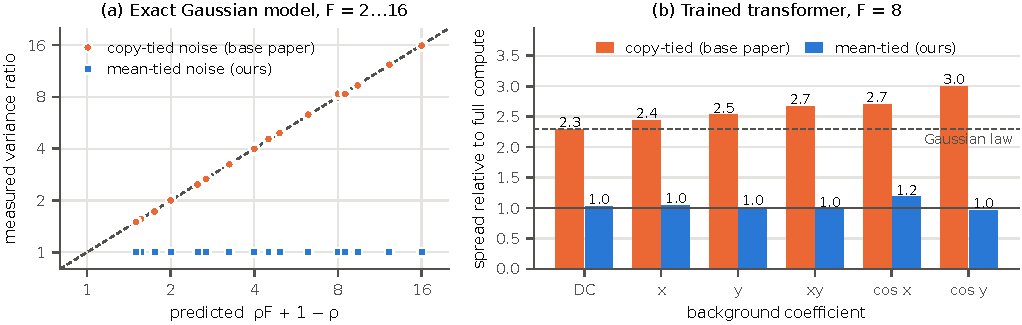
\includegraphics[width=0.82\textwidth]{../figures/fig_law.pdf}
\caption{The variance law. (a)~Exact Gaussian model: measured against predicted inflation of every background coefficient for $F\in\{2,4,8,16\}$ and three tied shares; mean-tied noise sits at 1. (b)~Trained standard model, oracle map: spread of the generated background coefficients relative to full compute.}
\label{fig:law}
\end{figure*}

\paragraph{Exact Gaussian model.}
We take the six-mode Gaussian background field of our data set (\S\ref{sec:trained}) as the whole clip, repeat it over $F\in\{2,4,8,16\}$ frames, and tie the starting noise on the top $100$, $75$ or $50\,\%$ of the rows.
The ideal denoiser is linear and known in closed form, so the 20-step sampler is exact.
Over all 72 coefficient--configuration pairs the measured variance inflation under \Copy{} matches Eq.~\ref{eq:law} within $\LawMaxRelErr\,\%$ (sampling error of 20{,}000 clips); for eight fully tied frames it is $\LawFEight$ against a predicted 8 (Fig.~\ref{fig:law}a).
Under \Mean{} the inflation is $1$ and the output equals the independent-noise output to \LawMeanMaxDiff.

\paragraph{Exact nonlinear denoiser.}
For a finite data set the ideal denoiser is a softmax-weighted average of the data~\cite{karras2022edm}, and the sampler lands on one of the clips.
We use $\IdealNData$ clips from our generator (smooth background, one or two moving sprites, a different static set in every clip, so this is the mixture case of Eq.~\ref{eq:mixture}) and $\IdealNSeeds$ noise seeds.
For each seed we record which clip independent noise produces, tie the noise on that clip's static set, and ask whether the sampler still produces \emph{that} clip (Table~\ref{tab:ideal}).

With \Copy{} it does so in $\IdealCopySame\,\%$ of runs, at $\IdealCopyPsnr$\,dB from the original, which is the 11--15\,dB the base paper reports; the backgrounds of the clips it lands on are $\IdealCopyStd\times$ as dispersed as they should be.
With \Mean{} it produces the original clip in $\IdealMeanSame\,\%$ of runs with a dispersion ratio of $\IdealMeanStd$.
The remaining runs are the mixture effect of Eq.~\ref{eq:mixture}; collapsing a few steps later removes it ($\IdealMeanSixSame\,\%$ at step 6, against $\IdealCopySixSame\,\%$ for \Copy{}).
A control separates the two things \Mean{} does.
Scaling the leader's noise by $1/\sqrt F$ gives the right \emph{variance} but not the right \emph{value}: the dispersion is correct ($\IdealColdStd$) and the sample is a different one ($\IdealColdSame\,\%$ same clip).
The variance fixes the distribution; taking the actual mean keeps the sample.

The 2-step draft is a poor map here.
An ideal denoiser at $t=0.5$ returns a blend of many clips, and no threshold reaches more than $\IdealDraftPrecision\,\%$ precision; forcing a moving position to be static changes the sample under either operator.
Reading the map from the trajectory a few steps later is far more reliable, and Theorem~\ref{thm:mean} makes that free.

\begin{table}[t]
\centering
\caption{Exact nonlinear denoiser on $\IdealNData$ clips, $\IdealNSeeds$ seeds, no network. ``Same clip'': the sampler lands on the clip that independent noise would have produced. ``Spread'': dispersion of the background coefficients of the produced clips relative to independent noise (1 is correct).}
\label{tab:ideal}
\small
\setlength{\tabcolsep}{3.2pt}
\begin{tabular}{@{}l c r rr rr@{}}
\toprule
 & & & \multicolumn{2}{c}{\Copy{} (base)} & \multicolumn{2}{c}{\Mean{} (ours)}\\
\cmidrule(lr){4-5}\cmidrule(l){6-7}
Static map & \makecell{tied at\\step} & \makecell[r]{tied\\(\%)} & \makecell[r]{same\\clip (\%)} & spread & \makecell[r]{same\\clip (\%)} & spread\\
\midrule
\tabinput{generated/table_ideal.tex}
\bottomrule
\end{tabular}
\end{table}
